% Source: Notion page “9. 增量学习机制”. Generated without rewriting its content.
\chapter{增量学习机制}

\section{增量学习总体设计}

校园行为识别系统在实际运行过程中会不断产生新的行为样本，其中包括新的场景数据、模型误识别样本、低置信度样本以及大小模型判断存在冲突的样本。如果模型始终使用初始训练数据进行训练，其识别能力将难以随着实际部署环境的变化持续提升。因此，本系统设计增量学习机制，使 Campus6 行为识别模型能够利用运行过程中持续积累的数据进行周期性更新。

考虑到 Campus6 当前仅包含六类校园行为，整体数据规模较小，本系统不采用持续在线更新模型参数的方式，而采用样本积累—难例挖掘—增量数据集构建—模型微调—模型压缩—评估发布的周期式增量学习流程。

整体流程如下：

\begin{figure}[htbp]
\centering
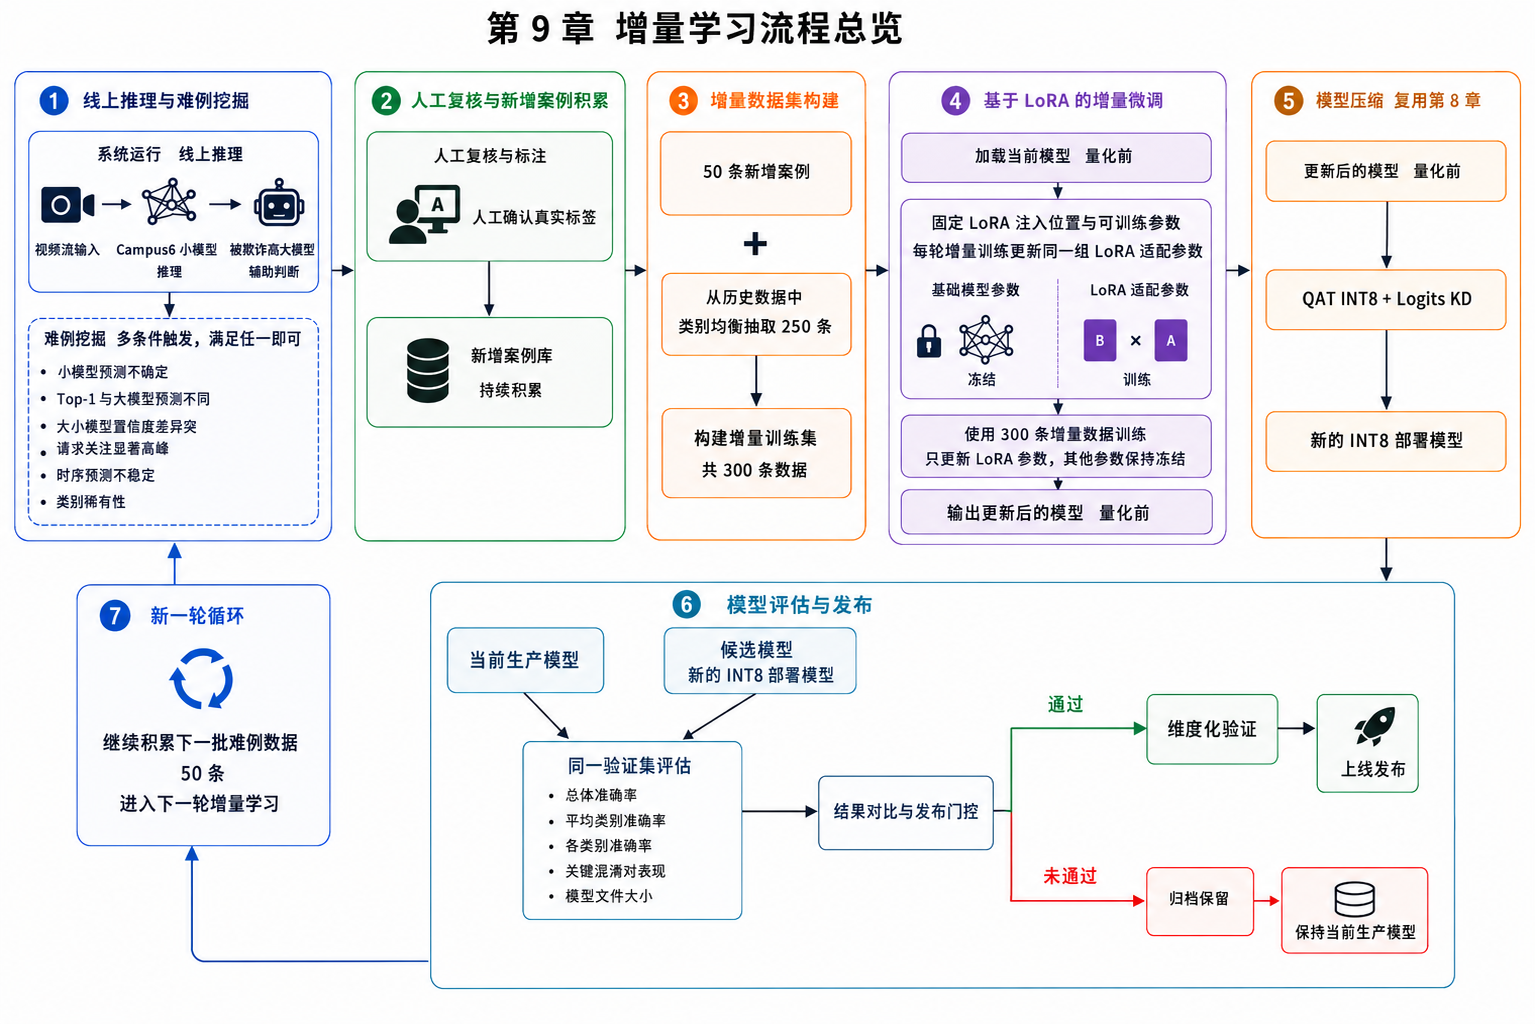
\includegraphics[width=0.96\linewidth,keepaspectratio]{figures/notion_image_06.png}
\end{figure}

注意，系统始终保留 FP32 Campus6 模型作为可持续训练的基础模型，因此，增量学习不会直接在已经量化的 INT8 模型上继续训练，而是首先更新 FP32 模型，再根据更新后的 FP32 模型重新生成对应的轻量化 INT8 部署模型。

这种方式将“模型能力更新”和“模型部署压缩”两个过程分离，使增量学习过程中始终能够在完整精度模型上进行参数优化，同时保证最终部署模型仍然满足系统对模型体积和推理效率的要求。

\section{难例挖掘与高价值样本发现}

并非所有新增数据都具有相同的训练价值。在系统实际运行过程中，大量正常行走、正常跑步等高置信度样本通常已经能够被 Student 模型正确识别，重复使用这些简单样本进行训练对模型性能提升有限。

因此，本系统重点从线上推理数据中自动发现当前模型识别能力较弱的困难样本（Hard Samples），将有限的人工审核和增量训练资源集中到更具有信息价值的数据上。

当前项目已经实现独立的难例挖掘模块。难例挖掘模块能够读取 Student 模型预测结果，并在存在 Teacher 推理结果时进一步结合 Teacher 信息计算样本难度。当前代码中的难例评分主要考虑以下因素：

\begin{enumerate}
\item 小模型预测不确定
当 Campus6 小模型 Top-1 与 Top-2 类别预测概率过于接近时，说明模型无法明确区分两个类别，将其标记为难例。

\item 大小模型预测不同
当 Campus6 小模型与视觉语言大模型对同一样本给出不同类别判断时，将其标记为难例。

\item 大小模型高置信度冲突
当大小模型分别以较高置信度判断为不同类别时，例如：

\[
l_push \leftrightarrow  conflict_push
\]

\[
l_chase \leftrightarrow  conflict_chase
\]

将其作为重点难例并优先进入人工复核。

\item 类别稀有
当某一类别当前样本数量明显少于其他类别时，该类别的新样本作为难例处理，以缓解类别不平衡。

\end{enumerate}

注：在4个因素之前，还有一个决定是否调用大模型的门控，也就是当小模型Top-1置信度高于0.3时，不调用大模型，不进入难例判断

一个样本可以同时满足多个难例条件，经过人工确认标签后的难例进入后续训练数据。

\section{增量数据集构建与采样策略}

系统将经过人工确认的难例作为新增训练数据持续积累。当新增难例累计达到 50 条时，启动一次增量训练。

每次训练时，从历史训练集中抽取 250 条样本，与 50 条新增难例共同组成固定规模的增量训练集：

\[
D_{inc}=D_{hard}^{50}\cup D_{history}^{250}
\]

因此：

\[
|D_{inc}|=300
\]

其中：

\begin{itemize}
\item 50 条新增难例用于强化模型对近期误识别样本和易混淆行为的学习；
\item 250 条历史样本用于保持模型已有的六分类识别能力，降低增量训练过程中的灾难性遗忘风险。
\end{itemize}

历史样本采用类别均衡采样，尽量保证 Campus6 六个行为类别均有样本参与训练，避免新增难例集中在少数类别时造成模型分类能力偏移。

因此，每轮增量训练统一采用：

50 条新增难例 + 250 条类别均衡历史样本

构成 300 条训练数据。

\section{基于 LoRA 的增量微调}

每当累计 50 条新增难例后，系统将其与从历史数据中抽取的 250 条样本组成 300 条增量训练集，并采用 LoRA（Low-Rank Adaptation） 对当前 Campus6 模型进行增量微调。

LoRA 冻结基础模型的大部分参数，仅通过低秩矩阵学习少量增量参数：

\[
\Delta W=BA
\]

模型更新表示为：

\[
W'=W_0+BA
\]

LoRA 在模型中的注入位置在首次配置后保持固定。后续每轮增量微调均更新同一组 LoRA 适配参数，不改变 LoRA 的作用层，也不解冻基础模型的其他参数。因此，每轮增量学习的可训练参数集合保持一致，只改变输入的增量训练数据。

相比全参数微调，LoRA 只更新少量且固定的参数，可以降低单次增量训练的计算成本，并减少不同批次新增数据对模型主体参数的大范围扰动。

同时，300 条训练数据中保留 250 条类别均衡的历史样本，使模型在重点学习最新 50 条难例的同时继续保持原有六分类知识，从而降低灾难性遗忘风险。

增量微调针对量化前的 Campus6 模型进行，微调完成后得到更新后的模型，再交由第 8 章的模型压缩模块生成新的 INT8 部署模型。

\section{增量训练触发与任务调度}

系统以累计 50 条新增难例作为一次增量学习的触发条件。

训练任务启动前，需要检查当前训练环境，包括：

\begin{itemize}
\item 新增难例数量是否达到要求；
\item 当前 FP32 模型 checkpoint 是否有效；
\item GPU 资源是否可用；
\item 是否已有其他模型训练任务正在执行。
\end{itemize}

只有满足全部条件后才启动本轮增量训练。训练成功后，已参与训练的 50 条难例被记录，系统继续累计下一批新增难例。

\section{模型评估、更新与回滚}

新生成的 INT8 模型作为 Candidate Model，与当前部署的 Baseline Model 进行对比评估。

主要评估：

\begin{itemize}
\item 六分类总体准确率；
\item 平均类别准确率；
\item 各类别准确率；
\end{itemize}

Candidate 模型只有在整体性能满足要求且不存在明显性能退化时才能替换当前生产模型。

如果评估通过：

\[
\begin{gathered}
\text{Candidate}\\[-0.2em]
\downarrow\\[-0.2em]
\text{Validated}\\[-0.2em]
\downarrow\\[-0.2em]
\text{Production}
\end{gathered}
\]

如果评估未通过，则保留当前生产模型，并归档本轮 Candidate。

